% -----------------------------------------------------------------------------
% Back matter for the IEEE Access manuscript
%
% Bibliography records belong in references.bib.
% This file contains only the bibliography command and author biographies.
%
% Verify time-sensitive roles, publication totals, memberships, and h-index
% values before final submission.
% -----------------------------------------------------------------------------

% -----------------------------------------------------------------------------
% References
% -----------------------------------------------------------------------------

\bibliographystyle{IEEEtran}
\bibliography{references}

% -----------------------------------------------------------------------------
% Stable compact biography command
%
% Arguments:
% #1 = photograph command
% #2 = author name
% #3 = opening text beside the photograph
% #4 = remaining text below the photograph row
%
% The photograph and opening text form one stable row. The remaining text
% is outside that row and may continue naturally across a column or page.
% -----------------------------------------------------------------------------

\newcommand{\accesscompactbio}[4]{%
    \par
    \addvspace{0.30\baselineskip}%
    \noindent
    \begingroup

    \setlength{\parindent}{0pt}%
    \setlength{\parskip}{0pt}%
    \emergencystretch=0.8em%

    % -------------------------------------------------------------------------
    % Photograph and opening biography text
    % -------------------------------------------------------------------------

    \begin{minipage}[t]{1in}
        \vspace{0pt}
        \centering
        #1
    \end{minipage}%
    \hfill
    \begin{minipage}[t]{\dimexpr\columnwidth-1.10in\relax}
        \vspace{0pt}
        \setlength{\parindent}{0pt}%
        \setlength{\parskip}{0pt}%
        \emergencystretch=0.8em%

        {\biographyheadfont\MakeUppercase{#2}\ }%
        {\biographyfont #3\par}%
    \end{minipage}

    % -------------------------------------------------------------------------
    % Remaining biography text
    % -------------------------------------------------------------------------

    \par
    \vspace{0.06\baselineskip}

    {%
        \biographyfont
        \setlength{\parindent}{0pt}%
        \setlength{\parskip}{0pt}%
        \emergencystretch=0.8em%
        #4\par
    }%

    \endgroup
    \par
}

% -----------------------------------------------------------------------------
% Qasim Mohamed Muhanna Alriyami
% -----------------------------------------------------------------------------

\accesscompactbio
{%
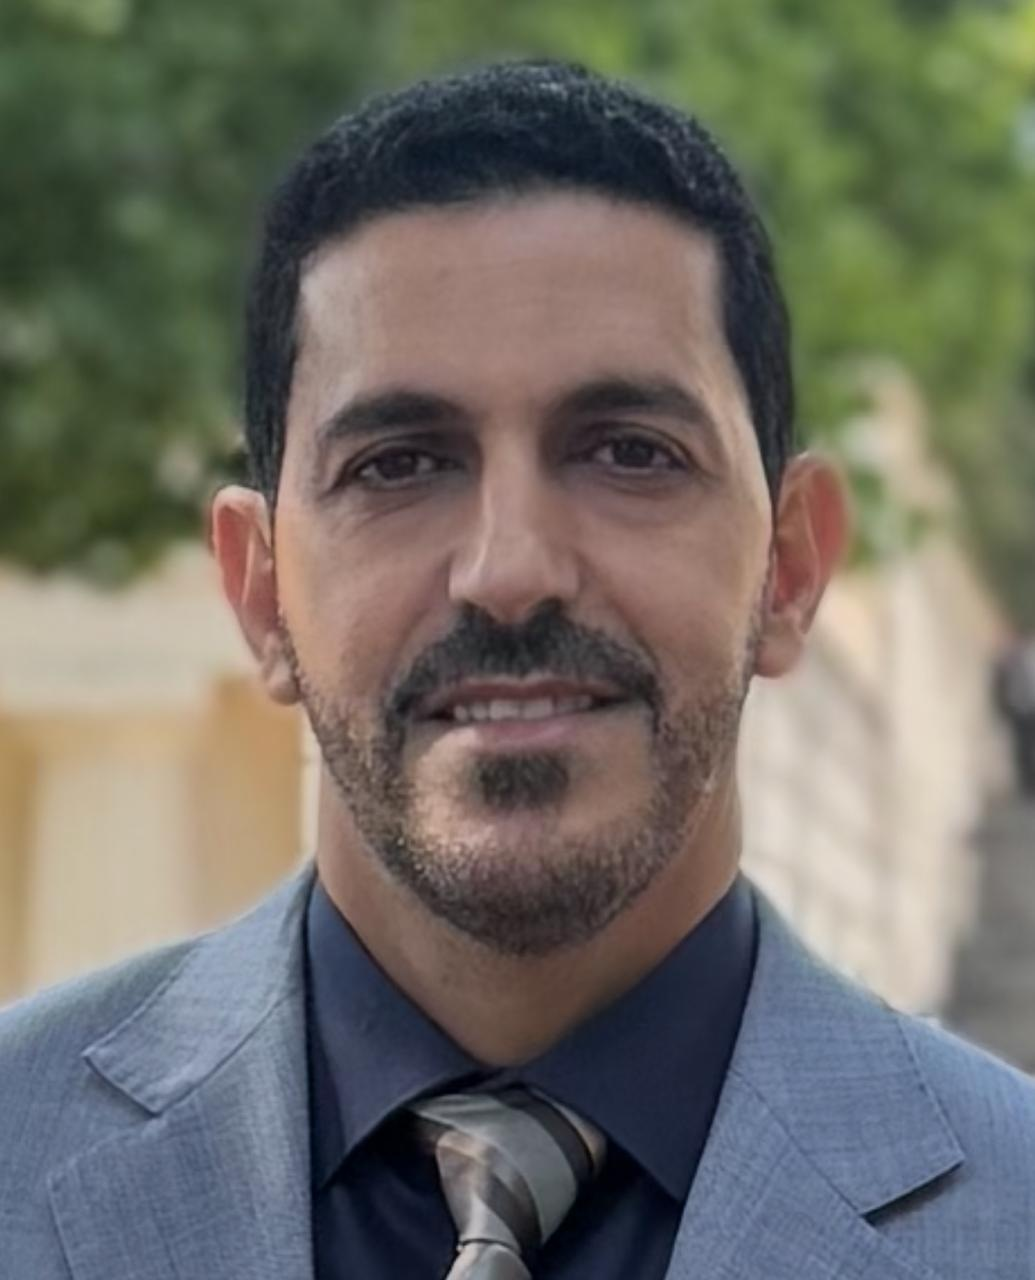
\includegraphics[
    width=0.95in,
    height=1.15in,
    keepaspectratio,
    clip
]{author_photos/qasim.jpg}
}
{Qasim Mohamed Muhanna Alriyami}
{%
received the B.Eng. degree in computer systems from the University of
Queensland, Brisbane, Australia, in 2006, the M.Sc. degree from the
University of Derby, Derby, U.K., in 2014, and the master's degree in
operational studies from the United States Army University, Fort
Leavenworth, KS, USA, in 2020.
}
{%
He is currently pursuing the Ph.D. degree in computer science at
Universiti Teknologi Malaysia (UTM), Johor Bahru, Malaysia. His research
interests include the application of artificial intelligence and machine
learning to cybersecurity, with a focus on insider threat detection,
behavioural modelling, temporal representation learning, and explainable
artificial intelligence.
}

% -----------------------------------------------------------------------------
% Mohd Murtadha Bin Mohamad
% -----------------------------------------------------------------------------

\accesscompactbio
{%
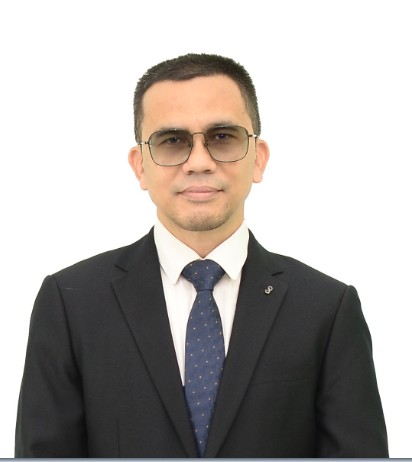
\includegraphics[
    width=0.95in,
    height=1.10in,
    keepaspectratio,
    clip
]{author_photos/murtadha.jpg}
}
{Mohd Murtadha Bin Mohamad}
{%
(Member, IEEE) is an Associate Professor and currently serves as the Ph.D.
Academic Programme Coordinator at the Faculty of Computing, Universiti
Teknologi Malaysia (UTM), Johor Bahru, Malaysia. He received the B.Eng.
degree in computer engineering from Universiti Teknologi Malaysia and the
M.Sc. degree in embedded systems and the Ph.D. degree in electrical
engineering from Heriot-Watt University, U.K.
}
{%
His research interests include robot motion planning, acoustic sensor
networks, and indoor positioning. He has supervised or co-supervised more
than 19 Ph.D. and 12 M.Sc. students and has authored or co-authored more
than 120 publications. His research profile includes a Scopus h-index of
13 and a Google Scholar h-index of 18.
}

\EOD